Before starting to establish a whole 3D mapping, a more simple case can be studied first and it will be shown, in this section, how to determine the distance to only one point. Indeed, the distance between the camera and a point of the target can be easily determined thanks to a little bit of trigonometry.

The context of this case is simple, the camera is recording images of the target while the artificial light source is projecting a point one the last one (see figure \ref{fig:schema1D}).

\begin{figure}[h]
  %\centering
  \centerline{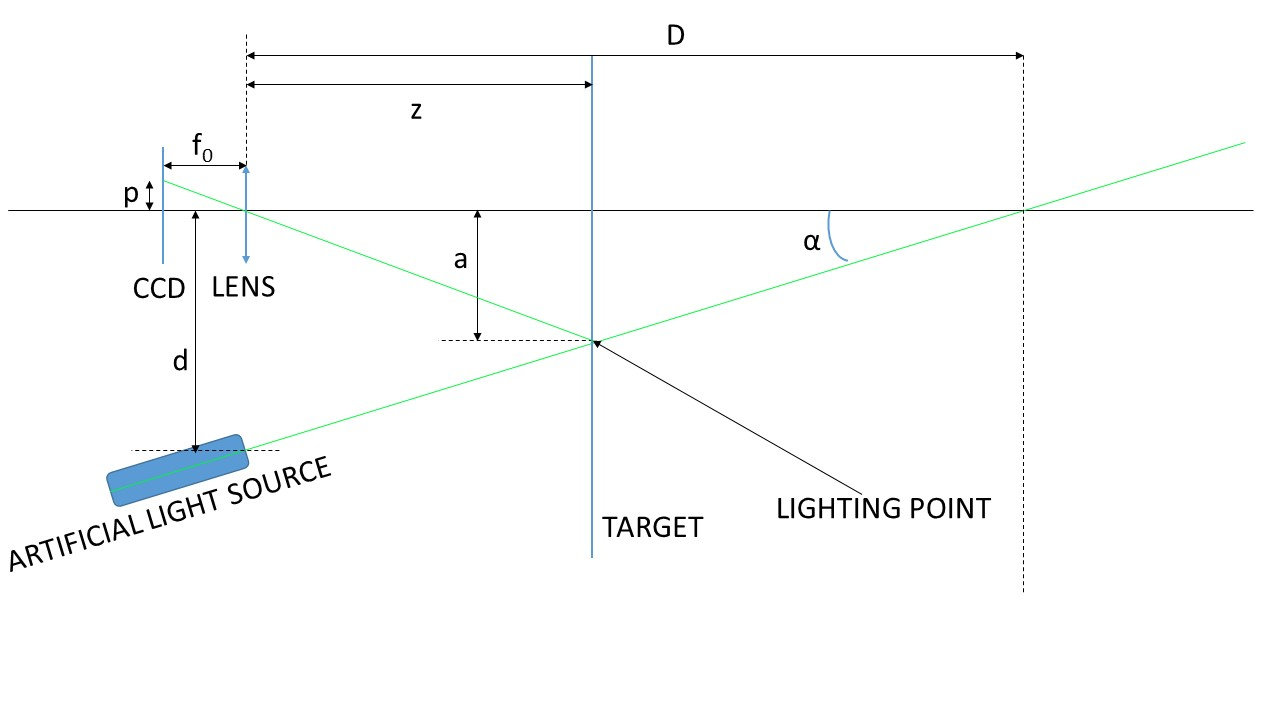
\includegraphics[scale=0.5]{fig/schema1D.jpg}}
  \caption{schema of the camera recording images of the target on which there is a lighting point from the artificial light source}
  \label{fig:schema1D}
\end{figure}

According to the figure \ref{fig:schema1D}, 
\begin{itemize}
\item \textbf{d} is the distance to determine.
\item $\bm{\alpha}$ is the angle between the focal axis of the camera and the focal axis of the light source.
\item \textbf{a} is the distance between the focal axis of the camera and the lighting point.
\item \textbf{D} is the distance between the camera and the lighting point when this one is on the focal axis of the camera.
\end{itemize}
Thus, we have

\begin{equation*}
	d=D-\frac{a}{\tan \alpha}
\label{eq:formule_1D}
\end{equation*}

However, $\bm{\alpha}$, \textbf{a} and \textbf{D} are not known yet, that is why a calibration phase is needed (see Figure \ref{fig:calibration}). The first parameter, $\bm{\alpha}$, is determined during the installation of the light source and the camera on the rover. Then, during the calibration, two steps can be identified. During the first one, a target is positioned such as the lighting point is on the center of the image recorded by the camera. Thus, \textbf{D} can be measured. During the second step, a target is positioned such as the lighting point is right on side (left or right) of the image recorded by the camera (see Figure \ref{fig:calibration}). Therefore, $a_0$ can be measured and we have

\begin{equation*}
	a = \frac{Na_0}{A_0}
\end{equation*}


with \begin{itemize} \item $N\ [pixels]$, the number of pixel between the center of the image recorded by the camera and the lighting point.
\item $A_0$ $[pixels]$, the number of pixel between the center of the image recorded by the camera and the lighting point during the calibration phase, that is to say, the half of the pixels of the width of the image.
\end{itemize}

Therefore, we have
\begin{equation}
	d=D-\frac{Na_0}{\tan \alpha}
\label{eq:formule1D}
\end{equation}

\begin{figure}[H]
  %\centering
  \centerline{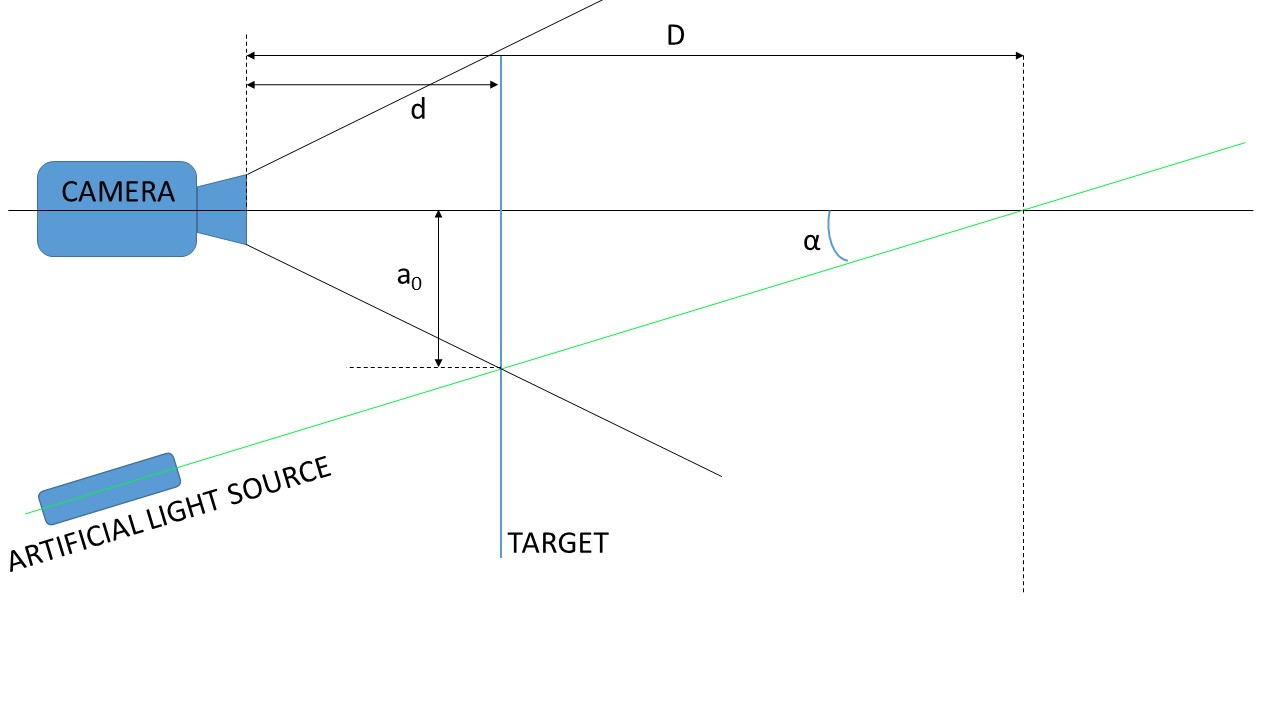
\includegraphics[scale=0.5]{fig/calibration.jpg}}
  \caption{schema of the calibration}
  \label{fig:calibration}
\end{figure}
